This chapter presents the formalisation of the policy emergence model.


% THE COMMON CORE
\section{Common core}

The common core is the centre part of the model which contains the concepts that can be placed in common for all policy making theories. The different parts of the common core are addressed here in the same order as they were addressed in the conceptualisation in \autoref{report_3Conceptualisation}.

%- PARAMETERS - The system and subsystems	
\subsection{The subsystems}

The policy arena is designed as a subsystem in this formalisation. This term is borrowed from the advocacy coalition framework and represents the arena in which all the actors interact and influence on another. Each subsystem contains the different rounds: agenda setting, policy formulation and world.

%- PARAMETERS - The agents
\subsection{The agents}

The model is composed of five types of permanent agents and one temporary agent. These are divided in two main categories: the agents considered as they have to spend resources to perform actions and the agents that are passive as all the actions they perform happen regardless of resources or of the situation. One agent fits in both categories.

%0
\paragraph{Active agents}

The active agents are the policy makers, the policy entrepreneurs and the external parties. Note that the external parties also have a passive role in which they provide the states from the truth agent, to the policy makers, the policy entrepreneurs and the electorate. This is considered to be a passive action as it is independent of resources.

The active agent's attributes are given as follows:

\begin{enumerate}

\item The \emph{active agent} is represented as an 10-tuple given by \texttt{agent = (ID, subsystem, type, beliefHierarchy, affiliation, advocacy, resources, coalition, team, networkStrategy)} where
\texttt{ID} is the unique ID of the agent,
\texttt{subsystem} is the subsystem ID in which the agent is present,  
\texttt{type} is the choice of agent type, 
\texttt{beliefHierarchy} is the agent's personalised belief hierarchy, 
\texttt{affiliation} is the political entity the agent identifies with,  
\texttt{advocacy} is the list of the issues the agent is supporting, 
\texttt{resources} is the agent's resources (a relative value), 
\texttt{coalition} is the coalition ID to which the agent is a member of, and 
\texttt{team} is the team ID to which the agent is a member of,
\texttt{networkStrategy} is the strategy that the agent will use for his/her networking actions.

\item A \emph{type} corresponds to a choice of agent. This can either be a policy maker, a policy entrepreneur or an external party. Depending on the type of agent, the actions will change from one agent to another.

\item The \emph{belief hierarchy} is made of two main parts: the agent's own belief hierarchy structure and associated values, and the belief hierarchies of all other agents and their values based on the agent's perceived knowledge of their beliefs (also referred as partial knowledge). The entire \emph{belief hierarchy} structure is therefore a list of belief hierarchies which is as long as the number of agents present in the model. The details of the hierarchy structure itself are provided later on.

\item The \emph{advocacy} is represented as a 4-tuple \texttt{(prob\_as, pol\_as, prob\_pf, prob\_as)} where \texttt{prob\_pf} is the problem chosen by the agent during the agenda setting process, \texttt{pol\_as} is the policy chosen by the agent during the agenda setting process, similarly \texttt{prob\_pf} and \texttt{pol\_pf} are the problem and policy selected by the agent during the policy formulation process. Note that some of these might not be used depending on the theories considered at any point. For the common core, only the problem is used.

\item The \emph{resources} are represented as a decimal on the interval [0, 1]. Resources are distributed to the agents based on their affiliation and on that affiliation's representation within the model. These resources are used by the agent to perform actions on other agents. The resources are relative amongst all agents.

\item The \emph{team} is represented as a 3-tuple given by \texttt{(team ID, belonging, strategy)} where \texttt{team ID} is the team to which the agent belongs, \texttt{belonging} is the agent’s feeling of belonging in a team and \texttt{strategy} is the agent's strategy when wanting to create a new team.  This attribute is only used in the three streams theory. The \emph{belonging} value relates to how much the agent feel (s)he is part of a team and defines the amount of resources the agent is willing to commit to his team. The \emph{strategies} refers to the strategy selected by the modeller for an agent when it comes to the creation of a team.

\item The \emph{coalition} is represented as a 2-tuple given by \texttt{(coalition ID, belonging)} where \texttt{coalition ID} is the coalition to which the agent belongs and \texttt{belonging} is the agent’s feeling of belonging in the coalition.

\end{enumerate}

%0
\paragraph{Passive agents}

The passive agents are the truth agent and the electorate. Both types of agents only perform passive actions.

\emph{The truth agent: } The truth agent is an agent not mentioned in the conceptualisation but required for the formalisation. This agent helps make the link between the world and the agents within the model. It gathers all the states of the world and provides them, as they are, to the external parties. One truth agent is present per subsystem. The only attribute of the truth agent is the belief hierarchy. This is a different one that for the active agents. It only contains the overall similar structure without any causal relations. Furthermore, it only contains the states for each of the issues.

\emph{The electorate: } The electorate represents the different constituencies within a subsystem. There are as many electorate agents as there are political affiliations in the model per subsystem. The role of the electorate is to influence the policy makers in their aims. The following defines the attributes of the electorate.

The \emph{electorate} can be given as a 6-tuple written as: \texttt{electorate = (ID, subsystem, affiliation, beliefHierarchy, representation)} where \texttt{ID} is the unique name of the electorate, \texttt{subsystem} considers in which subsystem it is, \texttt{affiliation} is its associated affiliation, \texttt{beliefHierarchy} is the associated belief hierarchy of the electorate and \texttt{representation} is the percentage of the total population which this electorate represents within the model. The sum of all \emph{representation} from all electorates must always be equal to 100. The \texttt{representation} parameter affects the amount of resources received by the agents in the model. The belief hierarchy of the electorate is similar in structure to the one of the truth agent. It only contains the issues.

%- PARAMETERS - The belief hierarchy
\subsection{Belief hierarchy}

The belief hierarchy is composed of two main parts: the issues and the causal relations. The issues are categorised in multiple layers: the deep core issues (the top layer), the policy core issues (the middle layers) and the secondary issues (the bottom layer). Secondary issues are linked to policy core issues through causal relations while policy core issues are linked to deep core beliefs through different causal relations. If multiple layers of policy core issues are present, each layer is also linked to each other with causal relations. The overall representation of this hierarchy structure is shown in \autoref{fig:Formalisation-04} for a three layered hierarchy.

Each issue is categorised by four parameters: the state, the aim, the preference and the awareness. The state defines the view of the agent of a certain issue as it is in the world. This view does not have to match reality and can be influenced by other agents. The aim shows what the agent would like to see happening in the world. The preference  which is a derived parameter, defines the urgency that the agent places on the each issues. It is calculated depending on the state of the issue, the aim of the agent and the causal relations linked to this issue. The sum of all preference weights on any single layer of the belief hierarchy have to be equal to 1. Finally, the awareness represents the fact that agents are aware of a specific issue or not. It can take the value of 0 or 1. If an agent is not aware of an issue, it will not consider it in any calculation as if it did not exist. The belief hierarchy structure also contains causal relations. These link the issues on the different layers of the structure. These are the representation, in the agent's mind, of how each of the issues are related to each other within the technical model and which issues affect which other issue.

\begin{figure}
\centering
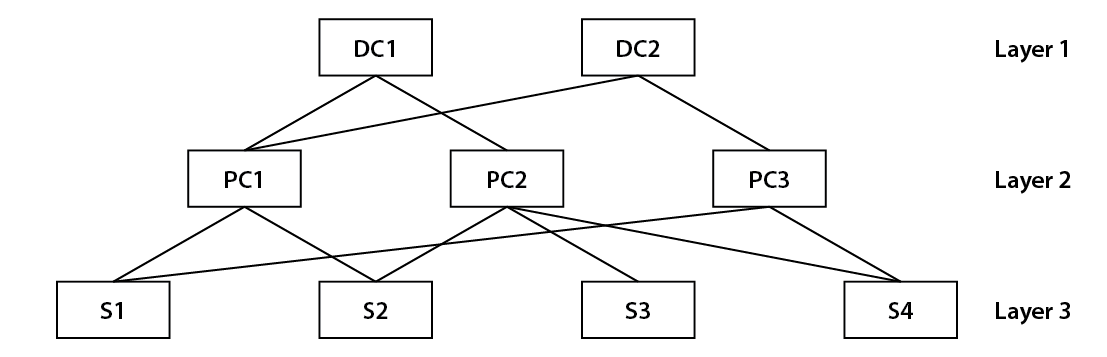
\includegraphics[scale = 0.75, angle = 0]{figures/Formalisation-04}
\caption{Example representation of a belief system with the three layers and several links between the layers. Not all possible causal relations are represented.}
\label{fig:Formalisation-04}
\end{figure}

Each agent has an attribute called \texttt{beliefHierarchy}. This attributes contains two parts as mentioned previously: the agent’s own belief hierarchy and the perceived hierarchies of all other agents in the model. It can be written as follows:

\begin{equation}
beliefHierarchy = [own_{hierarchy}, others_{hierarchy, n}]
\end{equation}

where $n$ represents the number of agents present in the model.

To further specify the hierarchy of the agent considered, the following can be said:

\begin{equation}\begin{split}
own_{hierarchy} &= [issues_k, causal\text{ }relations_l]\\
issues &= [state, aim, preference, awareness]
\end{split}\end{equation}

where $k$ defines the number of issues present in the belief hierarchy structure and $l$ the number of causal relations.

And it is also possible to specify the structure used to saved the perceived knowledge of the belief of the other agents:

\begin{equation}\begin{split}
other_{hierarchy} &= [issues_k, causal\text{ }relations_l]\\
issues &= [state, aim]
\end{split}\end{equation}

In both cases, the issues are specified with deep core issues first, policy cores following and ending with secondary issues. The causal relations are specified in the following example order: DC1-PC1, DC1-PC2, DC2-PC1, DC2-PC2, PC1-S1, PC1-S2, .... The state, preference and causal relation parameters are then specified on the interval of [-1, 1]. The preference is a percentage based parameters and is therefore calculated to be a number on the interval [0, 1].

%- PARAMETERS - The policy network
\subsection{Policy network}

The policy network is the network that links all agents within a subsystem. This network is composed of links with the following attributes: 

\begin{enumerate}
\item A \emph{policy network link} is represented as a 7-tuple \texttt{link = (agent1, agent2, awareness, awarenessDecay, conflictLevel)} where \texttt{agent1} and \texttt{agent2} are the agents at the end of a link, \texttt{awareness} is the awareness value, \texttt{awarenessDecay} is the decay value at which the awareness diminishes per time interval and \texttt{conflictLevel} is the conflict level characterising the relation between two agents for specific issues.

\item The \emph{awareness} value can take three main values. The value -1 refers to the fact that both agents are not aware of each other’s existence. They cannot network together without external introduction from a third party. For the value 0, the actors have no connection but know each other exist. They cannot network together until they have raised their awareness level to a non-negative value through networking actions. Any positive integer relates the value of awareness between the two agents. The awareness is given on the interval $]0,1]$. Note that awareness is relative amongst all links. The policy network links between policy makers can never be -1 as policy makers are public figures. Furthermore, a link cannot be downgraded to -1, it can only start at -1. As the awareness decays over time at a specific rate, there are several actions or events that can lead to a growth or stop the decay in the awareness between two agents. This is detailed later on.

\item The \emph{awareness decay} is represented by a 3-tuple \texttt{(value, time)} where \texttt{value} is the current value of the decay coefficient and \texttt{time} is a countdown. This countdown is by default set at 0, at which point decay of the awareness will happen. The countdown can be set at different values depending on actions that agents performed. The countdown will then go down to 0 every tick by 1. Whenever the countdown is not at 0, the decay is stopped.

\item The \emph{conflict level} parameter is determined for each agent for each issue's aim and state and for causal relations. Note that the conflict level between two agents will be difference depending on which agents is considered as the conflict level is obtained based on the perception of another agent's beliefs. The conflict level is therefore given as a 2-tuple for each link: \texttt{(agent 1, agent 2)}. Then for each agent, the conflict level is defined per issue for the state and then for the aim, and all causal relations. The conflict level is then calculated using:

\begin{equation}\begin{split}
CW \text{ }conflict \text{ } level_{n,n_m} &= |CW_n - CW_{n_m}| \\
aim \text{ } conflict \text{ } level_{n,n_m} &= |A_n - A_{n_m}| \\
state \text{ }conflict \text{ } level_{n,n_m} &= |S_n - S_{n_m}|
\end{split}\end{equation}

where $CW$ the causal weight, $A$ is the aim, $S$ is the state, $n$ is the agent for which the conflict level is calculated and $n_m$ is the perceived belief of agent $n$ on agent $m$ for that specific issue.

The resulting value is then formatted into a coefficient to be used in the grading of actions as is shown later on. When the result obtained is between 0 and 0.25, the conflict level is considered to be low, the coefficient is then set at 0.75. When the result obtained is between 0.25 and 1.75, the conflict level is considered to be medium, the coefficient is set to 0.85. Finally for a result higher than 1.75, the conflict level is considered high and the coefficient is set to 0.95. Note that both the intervals and the resulting coefficients can be varied by the modellers during experimentations to better tailor their model to their case studies.

\end{enumerate}

%-
\paragraph{Network upkeep and maintenance}

Each agent must maintain his/her policy network. For this, 20\% of agent’s resources can be used. The agents are allowed five actions, each time spending 4\% of the total amount of resources for each action. The order in which agents are selected to perform their network actions is random. These numbers can be changed by the modellers for the purpose of theirs cases.

Two strategies are differentiated for these actions. The modellers have to specified which strategy each agent uses in the model inputs. They are given as follows:

\begin{enumerate}
\item Largest network strategy - the agent will look into increasing his/her network as much possible:
	\begin{enumerate}
	\item The agent first wants to keep all links active. Any link that is below 30\% awareness level will be targeted for action. The lowest, but still above 0, will have priority.
	\item If all links are above 30\% awareness, the agent will look into introducing new links which had 0\% awareness. The priority is placed on the link with agents with the closest beliefs.
	\item If there are still resources left after step 1 and 2 are complete, the agent will maintain the links with the lowest awareness level in the network.
	\end{enumerate}

\item Focused network strategy - the agent will focus on maintaining a network of agents sharing its beliefs: (note that when it is stated similar belief, this relates to the problem that the agent is advocating for and no other issue)
	\begin{enumerate}
	\item The agent will look first for link where an agent with a similar belief (one of the agents has his belief within 0.2 of the other agent's aim belief) or higher belief level and with a awareness which is lower than 70\%. The agent will prioritise based only on the awareness level as long as the belief criteria is met.
	\item If no link qualifies, then the agent will seek to introduce new links in his/her network. The agent will select agents that have a similar belief or higher belief level.
	\item If both step 1 and 2 are met, the agent will look into maintaining an awareness level above 70\% for links still in service. The priority is put on the links with the lowest awareness value.
	\item If all previous steps are met, then the agent will simply look for new links with the priority placed on agents sharing his/her beliefs.
	\end{enumerate}
\end{enumerate}

The different actions mentioned above are performed as follows:

\begin{itemize}
\item An agent can increase the awareness in a network link if he feels the awareness level is too low. This awareness maintenance is dependent on three main parameters: the resources spent and the affiliation of both agents. The total increase in awareness for such an actions is calculated as:

\begin{equation}
awareness := awareness + resources \cdot affiCoef_{Aff_n,Aff_m}
\end{equation}

where the $affiCoef_{Aff_n,Aff_m}$ is the weight related to the affiliation of the two agents. If they share the same affiliation, then it is equal to 1.

\item Agents can also establish links with other agents for which they know they exist. This action can only be performed when the \texttt{link.awareness} parameter is equal to 0.

If this is the case, then the awareness can be increased through the spending of resources. The new awareness level is then calculated similarly to the awareness maintenance but with a small malus to account for the initial investment costs. The equation is given as follows:

\begin{equation}
awareness := resources \cdot affiCoef_{Aff_n,Aff_m} \cdot 0.5
\end{equation}

\item The notion of similar belief is defined as agents being close for the aim on issues at the policy core level. There are several steps to seek agents with similar beliefs:

\begin{enumerate}
\item Seek all links with awareness equal to 0 or higher and select their associated agents.
\item Select the aim parameter of the problem of the original agent.
\item For each associated agent, check its aim parameter for this same problem issue.
\item Calculate the difference of the parameter between the original agent and the associated agent for this issue.
\item Rank all differences from lowest to highest where the lowest is considered to be an agent of similar beliefs.
\end{enumerate}

This ranking is calculated based on the agent’s partial knowledge of other agent’s beliefs.
\end{itemize}

%- PARAMETERS - The affiliation network
\subsection{Affiliation network}

The affiliation network is a network that looks at the political affiliation of the different actors. Its links are represented as a 3-tuple given by \texttt{(affiliation1, affiliation2, affiCoef)} where \texttt{affiliation1} and \texttt{affiliation2} are the affiliations that are connected by the link and \texttt{affiCoef} represents the influence that an actor with an affiliation 1 can have on an actor with affiliation 2. The \emph{affiliation coefficient} is given on the interval $[0,1]$.

%- Actions
\subsection{The actions - Policy Makers}

There is a set of actions that policy maker agents can perform within the model. These actions are individual framing where the causal relations are the target of the influencing action, aim influence where the issue aim is the target of the influencing acton and state influence where the issue state is the target of the influencing action. These three times of actions are presented below in more details.

When selecting an action, the agent will perform all possible actions and calculate the likelihood grade of all actions. The agent will then select the action with the highest grade as the action to be implemented. The calculation of the likelihood of perfuming an action is mostly based on the beliefs of the influencing agent and his perception of the beliefs of the influenced agent. However, the actual impact of the action is based on the beliefs of the influencing agent and the beliefs of the influenced agent. This is an important difference that can sometimes justify why meaningless actions are performed. This can be due to a false perception of another agent’s beliefs.

%0
\paragraph{Individual framing}

The agents can attempt to influence the causal relation belief of other agents. This is an individual framing action. For this action, all causal relations related to the issue selected by the agent are considered. The likelihood to perform such an action depends on several parameters which are outlined below:

\begin{equation}
G_{CW, n_m} = conflictLevel_{CW, n, m} \cdot affiCoef_{Aff_n,Aff_m} \cdot awareness_{n,m} \cdot actionWeight_{n,m}
\end{equation}

where $G$ stands for the grade, $n$ is the influencing agent, $m$ is the influenced agent. $n_m$ is the perfection of the beliefs of the influenced agent by the influencing agent and $CW$ is the causal weight of the causal relation

If this action is selected, as it has the highest grade, then the impact of the action on the beliefs of the influenced agents is given by:

\begin{equation}
CW_{m} := CW_{m} + \left(CW_{n} - CW_{m} \right) \cdot resources \cdot affiCoef_{Aff_n,Aff_m}
\end{equation}

%0
\paragraph{Individual action - Aim change}

The agents can also attempt to influence the aim beliefs on the different issues of the hierarchy of other agents. The likelihood that such action be performed is obtained in a similar way as shown below:

\begin{equation}
G_{A, n_m} = conflictLevel_{A, n, m} \cdot affiCoef_{Aff_n,Aff_m} \cdot awareness_{n,m} \cdot actionWeight_{n,m}
\end{equation}

The impact of such action is then calculated with:

\begin{equation}
A_{m} := A_{m} + \left(A_{n} - A_{m} \right) \cdot resources \cdot affiCoef_{Aff_n,Aff_m}
\end{equation}

%0
\paragraph{Individual action - State change}

Similarly to the influence on the aims of an agent, the states can also be influenced. The likelihood of such an action being performed is given as follows:

\begin{equation}
G_{S, n_m} = conflictLevel_{S, n,m} \cdot affiCoef_{Aff_n,Aff_m} \cdot awareness_{n,m} \cdot actionWeight_{n,m}
\end{equation}

And the impact is calculated as follows:

\begin{equation}
S_{m} := S_{m} + \left(S_{n} - S_{m} \right) \cdot resources \cdot affiCoef_{Aff_n,Aff_m}
\end{equation}

%0
\subsection{Preference calculation (issues)}

As mentioned earlier on, the policy maker has a limited attention span. This results in having to select one issue at a time for which (s)he thinks is the most urgent issue. This urgency is defined as the preference of an agent and is calculated for each layer in the belief hierarchy of the policy maker. Two cases must be distinguished for calculating this urgency: whether the layer considered is at the top or in the rest of the hierarchy. The preference is calculated for each issue and the sum of all preferences on each layer must be equal to 1.

\paragraph{Preference calculation for the principle beliefs}

For the top layer which is composed of the principle beliefs, the preference is calculated differently than for the other layers. This is because these beliefs are on the highest layer and can therefore not be connected to higher layers with causal relations. The calculation of the preference for each issue is given by:

\begin{equation}
P_i = \frac{ |A_i - S_i|}{\sum_{j=1}^n |A_j - S_j|}
\end{equation}

where $j$ is defined at the number of principle belief issues and $i$ characterises the principle belief issue being selected for the calculation.

\paragraph{Preference calculation for the policy core and secondary beliefs}

The preference calculation for the other layers in the belief hierarchy is adapted to include the causal relations that link these layers to higher up layers. This calculation applies to the policy core beliefs which are in the middle of the hierarchy and the secondary beliefs at the bottom.

To calculate the preference, the gap between aim and state for the issues is considered along with the impact of the causal relation on the gap of the issue on the above layers. The causal relations are not always helping bridge the gap between the aim and the state of issues on a higher layer. If this is the case, then the causal relations are not considered within the calculation as there effort is counter productive within the mind of the agent. The resulting equation that can be used to calculate the preference for these layers is given by:

\begin{equation}\label{eq:preference2}
P_k= \frac{ |A_k - S_k| + \sum_{j=1}^n |CW_j \left( A_j - S_j \right)|}{\sum_{l=1}^p \left[ |A_l - S_l| + \sum_{j=1}^n \left|CW_{j,l} \left( A_{j,l} - S_{j,l} \right) \right| \right]}
\end{equation}

The sums only include these terms if $CW_j$ and $\left( A_j - S_j \right)$ have the same sign. If it is not the case, these terms are not considered. And where $p$ is defined at the number of policy core issues, $k$ characterises the policy core issue being selected for the calculation, $j$ specifies the associated deep core and $CW$ represents the weight of the causal relation.

Based on these preferences obtained, the agent will select one issue to advocate for as mentioned earlier. For each layer, the agent will choose the issue with the highest preference. This is the case for each layer. The actions that the agent will then perform will be to influence other agents on the issue they have selected specifically.

%0
\subsection{Partial knowledge and awareness decay}

The likelihood of performing an action is based almost entirely on the perception of an agent on another agent’s beliefs. This is also referred as the partial knowledge of an agent. This partial knowledge is the representation that agents have of other agent’s beliefs. To perform better informed decisions, the agents must update their partial knowledge about other agents.

This update is performed after two agents have interacted with one another. When an action is performed, both agents have come into contact and have learnt about each other’s beliefs on the issue they have interacted on. This allows them to gain knowledge about the other’s belief. Therefore, for each action implemented, each agent will have access to the belief of the other agent concerning the issue influenced during the action. This access is not complete, the agents will gain the beliefs of the other agent with a small uncertainty amount.

Furthermore, because the two agents have interacted, their awareness of one another will not decline. It is therefore kept at the current level for several time steps. Only after these time steps have passed and if both agents have not interacted since, the decay of their awareness of one another will continue.

%- PARAMETERS - The agenda parameters	
\subsection{Agenda and agenda selection}

The \emph{agenda} is a 1-tuple given by \texttt{agenda = (issue, problem, policy)} where \texttt{issue} is the issue that is placed on the agenda by the policy makers, \texttt{problem} is the problem selected and \texttt{policy} is the policy selected by the policy makers. Note that the problem and policy attributes are only considered within the three streams theory, they are left empty within the common core.


To constitute the agenda, an issue has to be chosen for the entire subsystem. For this two methods are proposed which can yield different results. The first method considers all the top issues as graded by the policy makers. They are affected by their normalised resources. The grade of each issue is the sum of all agent's resources which have chosen that issue as their preferred issue. Whichever issue has the highest grade becomes the issue on the agenda.

The second method used for the ranking and selection of the issues is similar to the first one. The difference is that here all issues are taken from each policy maker. They are then weighed all together (and not simply the issues at the top of the ranking of each agent). This approach is meant to represent a different approach to the power dynamics in the model. The grade for each policy is then obtained as:

\begin{equation}
rankingGrade = \sum_{i=0}^n \left( \frac{1}{P_{rank}} \cdot resources_n \right)
\end{equation}

where $n$ is the number of agents and $P_{rank}$ is the ranking of the policy for that agent.

The issue with the highest grade is then taken as the issue for the agenda.

%- Actions
\subsection{The actions - Policy entrepreneurs}

The actions of the policy entrepreneurs are the same as the ones presented for the policy makers. The only difference is that the policy entrepreneurs cannot choose the agenda.

%- Actions
\subsection{The actions - External parties}

As mentioned in the conceptualisation, the have a more complex roles that the policy makers and entrepreneurs. They have different and similar actions to these actors. Their first role is to transmit the states of the world to the different agents in the model. This role is passive and does not require any resources. The second and third roles that the external parties can perform are active roles. They perform actions on different agents which means that they require resources. The second role, blanket framing, is attributed 50\% of the total resources of the external party while the third role, blanket influence on the electorate, is attributed the last 50\% of the resources. These resources are then spent in intervals of 10\% of the total amount of resources on each of the actions. These resources values can be affected by the modeller decisions.

%0
\paragraph{Transmitting the states}


The states of the issue in the hierarchy beliefs of all agents are updated based on the information they get from the external parties. These external parties have access to the full and real states of the world. They can obtain these states from the truth agent which has the complete set of the states for each issue directly from the world. Each external party selects states that (s)he finds interesting to transmit them to other active agents. This transmission of the states can be affected by the political affiliation of the agents as agents of different affiliation are unlikely to fully trust one another. The equation used to calculate this update of the states is given below:

\begin{equation}
S_{agent} := S_{agent} + \frac{1}{n} \sum_{i=1}^n \left( \left(S_{EP_n} - S_{agent} \right) \cdot affiCoef_{Aff_n,Aff_m} \right)
\end{equation}

where $S$ stands for the issue state, $n$ is the number of external parties, $EP$ stands for external parties and $affiCoef_{Aff_n,Aff_m}$ is the affiliation related weight. The affiliation coefficient is the one that relates the affiliation of the agent and the affiliation of the external party selected. If an external party has not selected that specific state, then (s)he will not be able to provide the state for that issue. Furthermore, the external parties will only transmit the states to agents within their network. This can lead to some agents lacking states for specific issues because of the composition of their policy network.

%0
\paragraph{Blanket framing}

The external parties can also attempt to influence the understanding of the world of other external parties, the policy makers and policy entrepreneurs. The external parties perform such influence on all agents at the same time which leads to this action being called blanket framing. The overall calculation of the likelihood of performing such an action is similar to what was presented for the framing action of the policy makers. The impact is also similar but spread amongst all agents. Such action can only happen on the agents that are within the policy network of the external party. All causal relations related to the issue selected by the external party can be influenced.

The likelihood of performing a blanket framing action is calculated as follows:

\begin{equation}\begin{split}
G_{CW, n_m} &= conflictLevel_{CW, n, m} \cdot affiCoef_{Aff_n,Aff_m} \cdot awareness_{n,m} \cdot actionWeight_{n,m}\\
G_{CW, n} &= \sum_{m = 1}^{nagents-1} G_{CW, n_m}
\end{split}\end{equation}

where $CW$ is the causal weight selected, $n$ the external party performing the framing, $m$ the affected agents considered and $nagents$ the total number of agents.

The action on a causal relation for which the grade is the highest is then selected to be implemented. The causal relation of the affected agents are then given by the following equation:

\begin{equation}
CW_{m} := CW_{m} + \left( CW_{n} - CW_{m} \right) \cdot resources \cdot affiCoef_{Aff_n,Aff_m} \cdot \frac{1}{nagents}
\end{equation}

%0
\paragraph{Electorate influence}

Finally, the external parties can influence the goals of the electorate. This is done following the same template the goal influence of the policy makers and entrepreneurs. The only difference is that it is once again blanket influence which means that all electorate agents are affected at once. Note that because the external parties have a limited attention span, they can only influence the electorates on the issue they have selected. The impact of this influence is given by the following equation:

\begin{equation}
A_{El, i} := A_{El, i} + \left(A_{n, i} - A_{El, i} \right) \cdot affiCoef_n \cdot resources \cdot \frac{1}{nEl}
\end{equation}

where $n$ is the external party, $i$ is the issue and $nEl$ is the number of electorates.

%-
\subsection{Electorate passive action on policy makers}

The policy makers are passively influenced by the electorate. Each electorate has a certain affiliation to which policy makers are also related. Each policy makers' issue aim will be influenced by their respective electorate. This happens as a passive effect where the issue aims of the policy makers slowly progress towards the issue aims of the electorate. The equation to calculate the change in the aim of the policy maker is given as follows:

\begin{equation}
A_{PM} := A_{PM} + \left(A_{El} - A_{PM} \right) \cdot 0.001 \cdot \left| A_{El} - S_{El} \right|
\end{equation}

where $El$ stands for electorate and $PM$ for policy maker. Note that this is only performed for the issues of the policy maker for agents with matching affiliations. Furthermore, the value 0.001 is arbitrary and can be changed by the modeller depending on the case study.

%- PARAMETERS -  The policy instruments
\subsection{Policy instruments}

The policy instruments are measures that can are chosen by the policy makers to impact the real world. Policy entrepreneurs and external parties can also influence the policy makers in their choices. To assess the different policy instruments, the different active agents assess the impact of these instruments on the secondary issues in their belief hierarchy. These instruments have an impact on the gap between the states and the aim of each of these issues. The policy instruments can be described as follows:

\begin{enumerate}
\item A \emph{policy instrument} is represented as a 7-tuple \texttt{(name, impact, change, layer, children, awareness, feedback)} where \texttt{impact} is related to the impact of the policy on a specific issue, \texttt{change} is the objective change expected in the world due to this policy, \texttt{layer} corresponds to the layer in the instrument hierarchy (when used), \texttt{children} corresponds to the instruments linked to the selected instrument in the instrument hierarchy, \texttt{awareness} is related to the availability of the policy for a specific agent and \texttt{feedback} is related to the expected model feedback from the implementation of the policy considered.

\item The \emph{impact} of a policy instrument is given as a 2-tuple: \texttt{(issue, impact)} where \texttt{issue} defines which of the secondary issues is affected and \texttt{impact} specifies by how much.

\item The \emph{change} due to a policy instrument is the subjective representation of the impact of the policy instrument. These are the actual changes that will occur in the world with the implementation of the instrument. They are defined by the modeller and are fully independent on the agents.

\item The \texttt{layer} and the \texttt{children} are both parameters that related to the three streams theory. They are therefore outlined in that section and are left empty for the common core.

\item The \emph{awareness} parameter defines whether a certain policy instrument is known in a specific subsystem. This parameter is related to the diffusion theory and is further outlined in the section dealing with the diffusion theory.

\item The \emph{feedback} parameter contains the feedback effects as defined by the modeller. This parameter is related to the feedback theory and is further explained in the feedback theory section.
\end{enumerate}

%-
\subsection{Preference calculation (instruments)}

Similarly to the agenda setting round, in the policy formulation round, the agents have a limited attention span. They can therefore only select one policy instrument at a time. The calculations used to select these instruments are slightly different than the ones in the agenda setting. They are shown below

%0
\paragraph{Preference calculation}

The preference calculation of the secondary issues within the context of a policy formulation rounds are tweaked from the calculation presented in the agenda setting round. The main reason is that for the policy formulation, the number of issues considered is narrowed down by what is on the agenda. The agents can therefore only consider issues in the secondary belief layer that have a direct effect, according to their beliefs, on the issue that is on the agenda. All other issues are not included within the preference calculation. For the rest, \autoref{eq:preference2} is still used to calculate the preferences of the different issues for each agent according to their own beliefs.

%0
\paragraph{Instrument selection calculation}

Once the preferences for the different secondary issues have been attributed, it is possible to look at the preference of the instruments. These are used by the agents to assess the instruments and select the one they find most important. The equation that is used to calculate the preference of the different instruments is provided below. Similarly to the calculation of the preferences in the belief hierarchy, only instruments with impacts that have the same sign as the belief gap (aim minus state for a specific issue) are considered. The other instruments are counter productive and are therefore directly excluded from considerations.

\begin{equation}
P_i = \sum_{j=1}^n \left[ impact_j \cdot \left( A_j - S_j \right) \cdot P_j \right]
\end{equation}

where $n$ is the number of impacts this policy instrument has, and $j$ represents the secondary issue and the associated impact of the policy instrument on that issue.

Once all the preferences have been calculated, the agent will select the instrument with the highest preference. This will help define the actions that each agent can perform. Because no actions can be performed on the instruments directly, the agent will be able to perform actions on all issues directly related to the instrument and all causal relations which link the issue on the agenda and the issues related to this instrument. The likelihood and the impact of the actions are calculated in the same way as was shown previously. The aim here for the agents is to convince other agents that the instrument’s impact is as high as they perceive because their causal relations, aims and states beliefs are similar.

%-
\subsection{Policy instrument selection and implementation}

Similarly to the agenda setting round, the policy makers are the agents that can selected a policy instrument. Additionally, they will decide if a policy instrument should be implemented. This is done through one of two strategies which can be chosen by the modeller and which rare presented below.

%0
\paragraph{Unanimity}

If unanimity is required, all policy makers must have selected the same policy instrument for it to be implemented. If this is not the case, the instrument will not be implemented and the round will close without a definitive output.

%0
\paragraph{Majority}

If a majority is required, 50\% plus one policy maker must select the policy instrument for it to be implemented. The resources of the different policy maker has no impact on this majority as it had in the agenda setting round. If a majority cannot be found, the policy instrument will not be implemented.

%-
\section{External events}

The external events that are considered are external events that affect the agents. External events that would affect the world such as a flood for a hydrological model are of no interest and considered out of scope of this report. However, the impact on the model such as a change in the electorate composition due to the flooding is of interest.

The following is a non-exhaustive list of potential external events which the modeller could use.

\begin{enumerate}
\item An election - this would create a change in the electorate representation parameter which would in turn lead to different resources allocation for the policy makers.
\item The introduction of a new issue - a new issue could be introduced to the system or to a subsystem. This would affect the knowledge parameter for an issue for all agents present in the model.
\item Resources shift - a shift in the resources distribution due to an external event could be modelled. The way the resources are attributed could be modified to simulate a crisis situation were resources are scarce. This could also be modelled as a reduction in the possibility of actions (increasing the amount of resources that is spent per action).
parameter would be changed.
\item Policy network shifts - change in the awareness parameter of specific network links.
\item Affiliation network shift - change in the affiliation coefficient parameter that defines the interaction possibilities between two different political affiliations
\end{enumerate}

%-
\subsection{The model cycle}

For this formalisation, it is assumed that the different rounds are performed consecutively. First the agenda setting rounds are performed, then the policy formulation rounds and finally the real world. A further assumption is to assume that there is only one round of each of these steps is performed. This leads to a 3-step model with an agenda setting step, a policy formulation step and a world simulation step. The agenda which is obtained at the end of the agenda setting helps defines what the agents will be interacting about within the policy formulation.

This has several consequences. The first one is that the beliefs hierarchy of the agents must be a three-layer hierarchy. At the top are the principle beliefs, then in the middle the policy core beliefs and at the bottom the secondary beliefs. Within the agenda setting, the agenda decide on an agenda issue from the second layer, the policy core issues. Within the policy formulation, the agents select instruments which are related to the third layer.

The steps used to mode this approach are then detailed as follows:

\begin{enumerate}
\item World round:
	
	\begin{enumerate}
	\item \emph{World simulation:} The world which is an exogenous party to the model or an internal technical model are run to provide inputs for the next step.
	\item \emph{Trigger of external events:} Any event that the modeller decides to implement are activated at this stage of the model cycle.
	\item \emph{Update of the truth agent:} The technical output is converted into normalised data fitting with the issues present in the belief tree. These are placed in the truth agent's $S$ parameters.
	\item \emph{Electorate action on policy makers}
	\item \emph{Transmission of the states:} The external parties select their states of interest from the truth agent and pass the information to the agents within their policy network.
	\end{enumerate}
	
\item Agenda setting round:


	\begin{enumerate}
	\item \emph{Preference calculation (issues):} Each agent calculates the preference for their principle and policy core beliefs. The agents then each select an issue that (s)he will advocate for in his/her policy core beliefs based on the preferences calculated.
	\item \emph{Agent interactions:} 

		\begin{enumerate}
		\item \emph{Resources received:} Each active agent receives its resources based on his/her political affiliation.
		\item \emph{Network upkeep or maintenance}
		\item \emph{Belief influence actions:} All active agents perform their respective actions. The order in which the agents perform their actions is made random to not favour agents with first or last actions.
		\end{enumerate}

	\item \emph{Preference calculation (issues):} Each policy maker updates his preferences for his principle and policy core beliefs. This update of the preference is necessary to take into account the changes that might have occurred as a results of the agent interactions. Each policy makers choose the issue with the highest preference as their issue of preference.
	\item \emph{Agenda selection}
	\end{enumerate}
	
\item Policy formulation round:

	\begin{enumerate}
	\item \emph{Preference calculation (instruments):} Each agent update his preference for his secondary beliefs based on the issue on the agenda. Each agent then selects a policy instrument that (s)he will be advocating for.
	\item \emph{Agent interactions:} 

		\begin{enumerate}
		\item \emph{Resources received}
		\item \emph{Network upkeep or maintenance}
		\item \emph{Belief influence actions}
		\end{enumerate}

	\item \emph{Preference calculation (instruments):} Each policy maker upgrades their policy instrument preferences after the interaction step.
	\item \emph{Policy instrument implementation} 
	\end{enumerate}
	
\item \emph{The model advances:} The clock is advanced to the next tick. Programming of ticks actions are also performed (data collection, policy network awareness decay, …).

\end{enumerate}

% THE THREE STREAMS THEORY
\section{Three streams theory}

The three streams theory introduces a number of changes and additional concepts to the common core. These are detailed here. The first important addition and change is related to the policy instruments which are now assembled in an instrument hierarchy. Another change comes with the fact that the agent now must choose between a policy and a problem based on the calculated preference. Furthermore, because agents are not able to select policies, they are provided with an additional action. Finally, the agents can assemble in teams. This requires an algorithm for the creation of such teams and it brings in more actions that the actions can perform within and outside of their teams.

%-
\subsection{The policy instruments}

As explained in the conceptualisation, the actors now each have an instrument hierarchy similar to their belief hierarchy. To formalise this hierarchy, two attribute within the policy instruments are activated. These are the layer and children attributes. The layer attribute defines in which layer of the hierarchy the instrument fits. These layers are related to the layers present in the belief hierarch. This means that policy instruments in the second layer of the instrument hierarchy will have an impact on the issues which are in the second layer of the belief hierarchy. The children attributes helps understand which instruments are related across the different layers. This is defined by the modeller and is useful to navigate from one round to another. When a certain instrument is placed on the agenda from the second layer, then only his children present in the third layer can be considered by the agents. All other instruments are considered irrelevant. A representation of the instrument hierarchy is given in \autoref{fig:Formalisation-09}.

\begin{figure}
\centering
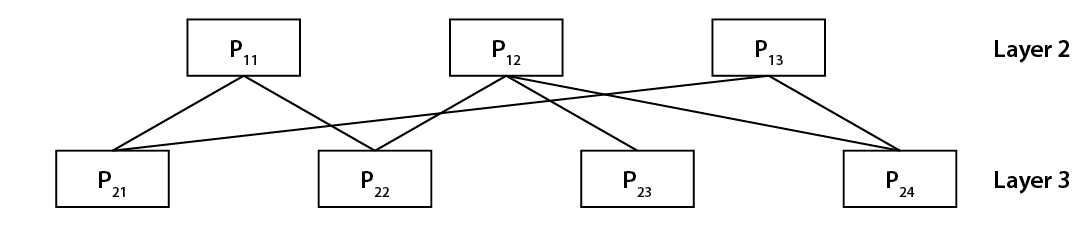
\includegraphics[scale = 0.75, angle = 0]{figures/Formalisation-09}
\caption{Instrument hierarchy representation with the two layers.}
\label{fig:Formalisation-09}
\end{figure}

There is an additional change that occurs within the policy instruments. The impact is not objective anymore. The impact is now a subjective parameters very much like the states and aims for the issues in the belief hierarchy. This is important as the agents will be able to influence other agents on their beliefs of the impact of the different instrument available to them.

%-
\subsection{Preference calculation (problems and policies)}

As mentioned within the conceptualisation, the agents can now select a policy or a problem. For that they must grade all problems and policies in every layer. They can then select the policy or problem that has the highest grade.

%0
\paragraph{Problem and policy preference calculation}

The problems and policy grades are obtained differently. The problems are based in the belief hierarchy and their grades are calculated similarly to the issues in the common core. The equation is given as:

\begin{equation}
G_{prob, i} = \left( A_i - S_i \right) + \sum_{j=1}^n \left| CW_j \left( A_j - S_j \right) \right|
\end{equation}

where $i$ corresponds to the policy core considered and $j$ the related deep core issues.

The policy instrument are assessed on their impact on the different gaps in their associated issues in the belief hierarchy. The equation used to calculate their grades is given by:

\begin{equation}
G_{policy, i} = \sum_{i=1} \left( A_i - S_i \cdot I_i \right)
\end{equation}

where $i$ corresponds to the policy core affect by the policy selected and $I$ is the impact expected from the policy.

Once all possible policies and problems have been graded, the agent will select the one with the highest grade. Then the process is repeated again but for the associated issues. This is done with only problems related to the policy selected if a policy was selected first or with the policies related to the problem selected if the problem was selected first.

The actions that the agents will perform will be based on whether they first selected a problem or a policy. These actions are detailed in a subsequent section.

%0
\paragraph{Agenda and agenda selection}

Within the three streams approach, the agenda selection is a little different than for the common core. The agenda is now composed of two parts: a problem and a policy. The issue attribute of the agenda is left empty. The rest is similar to the common. The problem selected for the agenda is the most popular problem for all agents considering their respective resources while the policy chosen is the most popular policy amongst all agents also considering their resources.

%0
\paragraph{Policy instrument selection and implementation}

For the policy formulation round, the procedure to select and implement a policy instrument is similar to the common core procedure. The policy chosen by all policy makers is considered. If a policy is beyond the threshold set but the modeller for implementation, the policy will be implemented. The problem chosen by the policy makers is not taken into account.

%-
\subsection{The actions (active agents)}

The influencing actions that the agents can perform are mostly similar to the ones in the common core. The main difference is that all their actions are performed on the problems if they have first selected a problem. The policy makers and entrepreneurs can perform framing, state influence and aim influence actions on other agents based on the problem they have selected in their belief hierarchy. The external parties can perform their blanket framing on other agents and blanket aim influence on the electorate. This is also based on the problem they have each selected.

For the agents that have selected a policy, an additional action is added. This action is an action that influences the impact beliefs of the policy instrument selected by the agent. For all agent, this action replaces the framing or blanket framing action. The aim and state influence actions remain the same. The likelihood of performing each action is calculated. Whichever action is most likely to be performed is implemented with a certain calculated impact.

The likelihood of performing a policy action is given as follows:

\begin{equation}
G_{I_{issue}, n_m} = conflictLevel_{I_{issue}, n, m} \cdot affiCoef_{Aff_n,Aff_m} \cdot awareness_{n,m} \cdot actionWeight_{n,m}
\end{equation}

where $n$ is the agent performing the action, $m$ is the agent on which the action is performed, $I$ stands for the impact that the action has on the mentioned issue. Note that if the instrument has an impact on four separate issues, then the agent will assess the likelihood of influencing each of the four impacts contained in that policy instrument.

The impact of the action is then given as follows:

\begin{equation}
I_{m, issue} := I_{m, issue} + \left( I_{n, issue} - I_{m, issue} \right) \cdot resources \cdot affiCoef_{Aff_n,Aff_m}
\end{equation}

where $n$ is the agent performing the action, $m$ is the agent on which the action is performed.


%-
\subsection{The teams} [Incomplete]


As mentioned in the conceptualisation, the three streams theory includes the concept of teams. This concept is formalised within this section.
Teams contain a number of agents that feel they share their beliefs for a specific issue. A team is therefore given as a 6-tuple written as: \texttt{(team ID, lead, members, issue, creation, resources)} where \texttt{lead} is the leader of the team (the agent that created the team), \texttt{members} is the list of members that are part of the team, \texttt{issue} is the policy issue that the team is advocating for (policy or problem), \texttt{creation} is the time at which the team has been created and \texttt{resources} consists of the resources at the disposal of the team to perform actions. The resources are calculated as the sum of all the members belonging level.

%0
\paragraph{Agent-team actions}

The agent-team actions are all actions that each agent performs to either decide to join or create a team. It also consists of actions related to the disbanding of teams and the checking that the team requirements are still met. Each agent goes through all of these actions each tick. Each agent can only be part of one team at a time in the agenda setting process and one team in the policy formulation process. Note that all actives agents can be part of teams. The following list presents the different actions that are taken in chronological order in which they are performed in the model: start a team, join a team, leave a team, disband a team and calculate belonging level.

%0
\paragraph{Start a team}

An agent that wants to start a team has to consider different requirements. Two different cases have to be considered here: the case where the agent first chose a problem and the case where the agent first chose a policy.

If the agent first chose a problem then the first requirement is that for the secondary issue chosen, the gap between aim and state must be above a certain threshold. This threshold is 0.8 in general but can be set to 0.5 in cases where a change in the magnitude of the state from the previous tick is larger than 0.5 (in case of an external event). This must be the case for all agents if they want to join the team. The second requirement relates to the belief states. For the agenda setting, it is the causal relation between the deep core issue with the highest preference for the starting agent and the policy core issue selected as the problem. For the policy formulation, the causal relation selected is the one relating the problem on the agenda and the secondary issue selected as the problem by the agent. All agents that want to join the team must be within 0.5 of the value of the causal relation for the agent starting the team.

If the agent first choses a policy, then there is a small change in the requirements looked at. The agent still looks at the gap requirement. However the second requirement is now dependent on the impact that the policy has on the secondary issues selected as the problem by the agent that is starting the team. The impact on the associated problem should be within 0.5 for the other agents considered to enter the team.

If both of these requirements are met, then the agents qualifies to join the team. Note that for each agent contacted, the agent starting the team loses 2\% of his resources and the contacted agent loses 1\% of his resources. This is to justify the resources needed for the exchange of knowledge. Furthermore, the agent starting the team will initially assess the other agents based on his knowledge of their beliefs. This leads to the spending of resources. If his perception of the other agent's beliefs are not true, then the agent will not join the team but the resources will have been spent regardless. The resources are also used to gain some information on the beliefs of the other agents. Even though the other agents might not be interested, spending these resources allow the agent to gain knowledge of the beliefs of the other agent within a certain range. Through this exchange of knowledge the agent also provides his own beliefs to the agent being contacted.

The creation of the team requirements are then based on the strategy that the agent is using. Two strategies are considered. The first strategy consists of starting a team with all the agents found that meet the requirements mentioned earlier. The team will then be composed of the maximum number of agents possible. The second strategy consists of starting a team once a certain number of agents has been established to meet the aforementioned requirement.

Upon the creation of a team, all agents that are part of the team are added to the member list. The lead agent of the team is the agent that started the team. Each agent's belonging level is also calculated based on a weighted average of the beliefs of the team on the state of the issue advocated for. Joining a team will also lead to the half of the awareness decay in the links between the agents present in the team, effectively counting as an action.

%0
\paragraph{Join a team}

An agent can join a team if (s)he is not already part of a team. For this, the agent will check the same requirements as when creating a team (gap and causal relation/impact requirements). This is done for the issue of the team (s)he is approaching. For each team that the agent probes, 2\% of his resources are spent. If the requirements are met, then the agent will join the team and be added as a member of the team. The agent is allowed to spend 50\% of his resources for such a search. Once these resources have been depleted or all team have been considered, the agent moves on.

%0
\paragraph{Leave a team}

An agent can leave another team for one reason: because his belonging level is too low. The belonging parameter of the agent is checked every time period. If it descends below 30\% then the agent will automatically leave the team. If the team remaining has less than three agents, it will be disbanded right away. Note that the belonging parameter is updated based on the perception of an agent on another agent's beliefs (partial belief) without full knowledge. This will artificially increase the life of teams. 

%0
\paragraph{Disband a team}

As mentioned earlier, a team will be disbanded if the problem or policy advocated by the team does not match the problem or policy advocated by the lead agent. This can be due to the leader being influenced and having changed his/her preferences. This is checked every five time periods. The second reason for which a team will be disbanded is if the agents present in the team to not meet the team creation requirements anymore. This is also checked every five time periods.

%A team can be disbanded if the lead agent in the team changes his advocacy parameter for which the team was created. This is checked every time period. A team can also be disbanded if the thresholds creation criteria are not met. This is checked every five time periods.  For this, the lead agent checks whether the other agent's are within 0.2 of his beliefs for the advocated issue. If they are within that threshold, then the team will remain. This check does not costs resources and is based on the lead agent's perception of the knowledge of the other agents. It does not require a knowledge exchange.

%0
\paragraph{Belonging level setting}

The belonging level in a team is used to measure how much resources an agent is willing to contribute to the team resources and how much (s)he will keep for his own individual belief influence actions. This belonging level is entirely related to the problem or the policy being advocated by the team.

The belonging level is obtained differently depending on whether the team has selected an problem or a policy. For a problem, the belonging level is obtained through the problem that is being advocated by the entire team. The steps are shown below:

\begin{enumerate}
\item The weighted average of all agent’s belief on the state of the problem being advocated by the team of all agent is calculated using:
	\begin{equation}
	S_{prob, weighted} = \sum_{i=1}^n resources_n \cdot S_n
	\end{equation}

	Note that this weighted average might be difference for each agent as it is based on partial knowledge and not full knowledge. The belonging parameter will be affected by the perception of other agent's beliefs.

\item The belonging level is then calculated using the following equation:
	\begin{equation}
	Belonging = 1 - \left| S_{prob,agent} - S_{prob,weighted} \right|
	\end{equation}
\end{enumerate}

The belonging level in a team that is advocating for a policy is different. It is calculated using the impacts that the policy has on the different issues in the belief hierarchy. The belonging level of each agent is calculated as the difference between his/her own total belief and the average of the other agent’s total beliefs. The ‘total belief’ of each agent is calculated for the policy that is being advocated by the team according to the agent’s own beliefs as the sum sum of the absolute value of all impact that policy has. To estimate the total belief of other agents, agents have to rely on their partial knowledge. The steps are provided below:

\begin{enumerate}
\item The total belief of all agents is calculated:
	\begin{equation}
	TB_{pol, m} = \sum_{i=1}^p |I_{n_m, issue}|
	\end{equation}
	where $m$ is the agent being considered, $n$ the agent performing the estimation of the total belief and $p$ the number of impacts that the policy instrument has.

\item The average of the other agent’s total belief is calculated:
	\begin{equation}
	TB_{pol, avg} = \sum_{i=1}^p |TB_{pol,m}|
	\end{equation}

\item The belonging level is then calculated using the following equation:
	\begin{equation}
	Belonging = 1 - \left| TB_{pol,m} - TB_{pol, avg} \right|
	\end{equation}
\end{enumerate}


%-
\paragraph{Team belief actions}


Once the teams have been constituted, these teams must perform actions. These are the belief actions. There are two types of actions that the team can conduct. They can first perform intra-team actions to help the team get more consistent beliefs. They can also perform inter-team actions. In this case the aim is to convince other agents outside of the team that the belief of the team are more important. Each type of actions uses 50\% of the resources reserved for the team. These actions are performed in intervals of 10\% of the total amount of resources reserved. The resources available to team are equal to the sum of the belonging attributes for each of the members of the team.


\begin{itemize}


\item Intra-team actions:


There are four main intra-team actions: blanket framing on causal relations, blanket framing on policy instrument impact, direct influence on aim and direct influence on state beliefs. The aim for these actions is to help the entire team be a more coherent entity with agents having similar beliefs regarding the issues they advocate for. As each of the team is based on awareness between the different agents, each agent has a say on which action should be chosen. Therefore each agent assesses all of the possible actions based on the partial knowledge he has of the other agents in the team. Because the agents are in a team, they all know fairly well the beliefs of the others in the team.


Within the context of a team, these actions are performed by the team leader. Considering that the agents are all in the same team, they all know each other's almost exact beliefs and it therefore does not matter who decides on which action to take as the results will be the same.


The blanket framing action on causal relation is used in the case where the team has selected a problem as the issue it is advocating for. This action is calculated using the following equation for each agent and for each causal relation:


\begin{equation} \begin{split}
 \Delta CW_{agent} &=  conflictLevel_{n,m} \cdot affiCoef_{n,m} \cdot awareness_{n,m} \cdot actionWeight_{n,m} \\
 G_{n,framing} &= \sum^{nagents}  \Delta CW_{agent}
\end{split}\end{equation}


The blanket framing action on the policy impact is  used in the case where the team has selected a policy as the issue it is advocating for. This action is calculated using the following equation for each agent and for each impact:


\begin{equation} \begin{split}
 \Delta I_{agent} &=  conflictLevel_{n,m} \cdot affiCoef_{n,m} \cdot awareness_{n,m} \cdot actionWeight_{n,m} \\
 G_{n,framing} &= \sum^{nagents}  \Delta I_{agent}
\end{split}\end{equation}


The state influence action is calculated using the following equation for each agent and for each issue:


\begin{equation} \begin{split}
\Delta S_{n} &=  conflictLevel_{n,m} \cdot affiCoef_{n,m} \cdot awareness_{n,m} \cdot actionWeight_{n,m} \\
 G_{n,state} &= \sum^{nagents}  \Delta S_{n}
\end{split} \end{equation}


where agent $1$ is the agent performing the action and $n$ is the agent being influenced.


The aim influence action is calculated using the following equation:


\begin{equation} \begin{split}
\Delta A_{n} &= conflictLevel_{n,m} \cdot affiCoef_{n,m} \cdot awareness_{n,m} \cdot actionWeight_{n,m} \\
 G_{n,aim} &= \sum^{nagents}  \Delta A_{n}
\end{split}
\end{equation}


where agent $1$ is the agent performing the action and $n$ is the agent being influenced.


For each of these actions, the grade is the sum for all agents of the action as these are intra-team actions. The total grades for each are compared and the one with the highest impact is selected to be implemented.


The actual change in the agents impacted is then given by the following equations:


\begin{equation} \begin{split}
CW_{agent} &:= CW_{agent} +  \left(CW_{avg} - CW_{agent} \right) \cdot affiCoef_n \cdot resources \cdot \frac{1}{nagents} \\
I_{agent} &:= I_{agent} +  \left(I_{avg} - I_{agent} \right) \cdot affiCoef_n \cdot resources \cdot \frac{1}{nagents} \\
S_{n} &:= S_{n} + \left(S_{1} - S_{n} \right) \cdot resources \cdot affiCoef \cdot \frac{1}{nagents} \\
A_{n} &:= A_{n} + \left(A_{1} - A_{n} \right) \cdot resources \cdot affiCoef \cdot \frac{1}{nagents} \\
\end{split}\end{equation}




\item Inter-team actions


There are also four inter-team actions: framing on causal relations, framing on policy impact, direct influence on aim and direct influence on state beliefs. The aim for these action is to influence the belief of individual agents present outside of the team. These actions are graded by each of the agents present in the team and the action that has the most merit from all actions of all the agents is the one selected by the team as a whole. To benefit better from the team, the agents can count on the overall team network and the team resources. The framing on causal relation is performed if the team has chosen a problem as its issue while the framing on policy impact is for when the team has chosen a policy as its issue.


To better benefit from the team network, a shadow network is established between the team and all agents outside of the team. The awareness for the established links is equal to the highest found between one of the agents in the team and the outsider agent. Furthermore, the conflict level between the team and this agent is calculated for the issue of the team based on the average beliefs of the team and the outsider agent's beliefs. The links behave similarly to the normal links between the agents.


Each of the actions are performed using 10\% of the resources of the team and using the partial knowledge of the agents within the team. As mentioned before, the awareness and conflict levels are obtained through the team-outside agent links.


The framing on causal relation grade is obtained using:


\begin{equation}
CW_n :=  CW_n + \left(CW_{n} - CW_{n_m} \right) \cdot resources \cdot awareness_{team,m}  \cdot actionWeight
\end{equation}


where $m$ is the outsider agent and $n$ is the agent within the team.


The framing on policy impact grade is obtained using:


\begin{equation}
I_n :=  I_n + \left(I_{n} - I_{n_m} \right) \cdot resources \cdot awareness_{team,m}  \cdot actionWeight
\end{equation}


The state and aim influence action grades are obtained using:


\begin{equation}
S_n :=  S_n +  \left(S_{n} - S_{n_m} \right) \cdot resources \cdot awareness_{team,m}  \cdot conflictLevel  \cdot actionWeight
\end{equation}


\begin{equation}
A_n :=  A_n + \left(A_{n} - A_{n_m} \right) \cdot resources \cdot awareness_{team,m}  \cdot conflictLevel  \cdot actionWeight
\end{equation}


where $m$ is the outsider agent and $n$ is the agent within the team.


All of the actions are performed and then the agents update what they believe will be the new beliefs after the actions. The actions that results in the smallest difference between the preference of the team and the preference of the agent influenced for the policy or problem advocated by the team will be chosen to be implemented.


When the actions are performed, the following equations are used to obtain the final values of the beliefs:


\begin{equation} \begin{split}
CW_m &:=  CW_m + \left(CW_{n} - CW_{m} \right) \cdot resources \cdot awareness_{team,m} \\
I_m &:=  I_m + \left(I_{n} - I_{m} \right) \cdot resources \cdot awareness_{team,m} \\
S_{m,state} &:=  S_{m,state} + \left(S_{n} - S_{m} \right) \cdot resources \cdot awareness_{team,m} \\
A_{m,aim} &:= A_{m,aim} + \left(A_{n} - A_{m} \right) \cdot resources \cdot awareness_{team,m} 
\end{split}\end{equation}


\end{itemize}


%-
\subsection{Note on the agent individual belief actions}


The agent can also perform actions as a simple individual regardless of being in a team or not similarly to the actions performed in the backbone+ model. The resources used to this effect are the resources left depending on the belonging parameter if the agent is in a team. If the agent is team-less, then all his resources left after the agent-team actions are the resources can be used.


The actions that the agent can perform are dependent on whether he has first chosen a policy or a problem similarly to the inter-team actions. In both cases, the agent can perform a state and aim influence action on other agents. Furthermore, if the agent has first chosen a problem, he will be able to perform a framing on causal relation action while if the agent had first chosen a policy, he will be able to perform a framing on impact action. The process and equations used are the same as the ones presented in the inter-team actions section.




%0
\subsection{The model cycle} [Complete]


The model cycle used when the three stream theory is considered is given below. The parts that are common to the common core are not detailed but they are repeated for a better understanding.


\begin{enumerate}
\item World round:
	
	\begin{enumerate}
	\item \emph{World simulation}
	\item \emph{Trigger of external events}
	\item \emph{Update of the truth agent}
	\item \emph{Electorate action on policy makers}
	\item \emph{Transmission of the states}
	\end{enumerate}
	
\item Agenda setting round:


	\begin{enumerate}
	\item \emph{Preference calculation (problems and policies):} Each agent calculates the preference for their principle and policy core beliefs (policy and problem). The agents then each select a problem or a policy that (s)he will advocate for in his/her policy core beliefs based on the preferences calculated.
	\item \emph{Agent interactions:} 


		\begin{enumerate}
		\item \emph{Resources received}
		\item \emph{Agent-team actions:} Each agent can decide to join or start a new team depending on his belief and his choice of policy or problem.
			\begin{enumerate}
			\item \emph{Belonging parameter update:} If an agent is in a team, then its belonging parameter is updated based on the latest beliefs. 
			\item \emph{Leave a team:} An agent will leave a team of his own accord only for one reason: if the belonging level drops below 30\%. If the agent leaves the team he was part of, the team must then be checked to see if it has enough members. If it has less than three members it will have to be disbanded and all agents present in the team are removed from it.
			\item \emph{Disband the team:} If the agent is the lead of the team, there is a possibility that he will disband the team. This happens when the policy issue the agent is advocating for changes and does not match the issue of the team anymore. This is checked every five ticks. If they do not match, the team will be disbanded and all agents removed from the team. The requirements used to create a team are also checked every five ticks to see if the members should still be in the team. If the number of members falls below three during this review process, then the team will be disbanded.
			\item \emph{Join a team:} If the agent is not in a team, he will first try to join an existing team. For each team considered, he will spend a small amount of resources to gather information. If the gap in his beliefs is above the required thresholds for the issue that the considered team is supporting, and his state belief are closed enough to the team's leader state belief on that issue, then the agent can join the team.
			\item \emph{Create a team:} If the agent has not managed to join a team, then he has the possibility to create a team himself. For this the agents looks towards the agents to which he is connected and has awareness. If the agent first chose a policy, then the agent will be able to start a team around that policy only. The same is true if the agent had chosen a problem. For each of these agents, the agent considers the gap in this issue along with the state to see if he shares beliefs with the other agents. Considering each agents costs a little resources for both the agent searching and the agents he is interacting with. Then depending on the personal strategy of the agent, the agent creates a team with all the agents he has found or he creates a team once he has found a sufficient amount of agents.	
			\end{enumerate}
		\item \emph{Team actions:} Each team performs their intra-team actions followed by their inter-team actions.
		\item \emph{Network upkeep or maintenance}
		\item \emph{Belief influence actions:} All active agents perform their respective actions based on their remaining resources.
		\end{enumerate}


	\item \emph{Preference calculation (problems and policies):} Each policy maker updates his preferences for his principle and policy core beliefs. This update of the preference is necessary to take into account the changes that might have occurred as a results of the agent interactions. Each policy maker then chooses first a problem or a policy with the highest preference as their issue of preference. They then select its associated policy or problem.
	\item \emph{Agenda selection}
	\end{enumerate}
	
\item Policy formulation round:


	\begin{enumerate}
	\item \emph{Preference calculation (problems and policies)}
	\item \emph{Agent interactions:} 


		\begin{enumerate}
		\item \emph{Resources received}
		\item \emph{Agent-team actions}
		\item \emph{Team actions}
		\item \emph{Network upkeep or maintenance}
		\item \emph{Belief influence actions}
		\end{enumerate}


	\item \emph{Preference calculation (problems and policies)}
	\item \emph{Policy instrument implementation} 
	\end{enumerate}
	
\item \emph{The model advances}


\end{enumerate}




% THE ADVOCACY COALITION FRAMEWORK
\section{The advocacy framework coalition}


%- PARAMETERS - The coalitions
\subsection{Coalitions}


\textcolor{red}{This will probably be updated later.}


The coalitions are created following the three streams theory.  They contain a number of agents that feel they share their beliefs for a specific issue. A team is therefore given as a 6-tuple written as: \texttt{(team ID, lead, members, issue, creation, resources)} where \texttt{lead} is the leader of the team (the agent that created the team), \texttt{members} is the list of members that are part of the team, \texttt{issue} is the policy issue that the team is advocating for, \texttt{creation} is the time at which the team has been created and \texttt{resources} consists of the resources at the disposal of the team to perform actions. The resources are calculated as the sum of all the members belonging level. It is therefore a number that can be above 1.




This section presents the model of the backbone and the backbone+ model combined to the advocacy coalition framework but excluding the three streams theory. The items that are similar to what is presented in the previous section are not re-explained. Note that several key elements from introduced in the three streams theory are also used for the advocacy coalition framework. They are not re-explained.


The ACF model is very similar to thebackbone+ model. The main difference relates to the addition of coalition to which agents are assigned. These coalitions are formed based on a deep core belief that was selected by the modeller as the deep core around which the coalitions should be assembled. Coalitions are formed fundamentally differently than the teams within the three streams theory. However, they still have a leader and are still advocating for an issue. The difference relates in the fact that agents are assigned to them depending on their deep core beliefs and regardless of their policy core or secondary beliefs. Note that the coalitions used for the agenda setting process are different than the coalitions that are used at the policy formulation level. These are considered as two different arenas due to the different levels of aggregation.




%-
\subsection{Coalition creation}


There are several algorithms that can be used to create coalitions. One is proposed here. First the leader of any potential coalition is selected. This is done by selecting the agent with the most amount of awareness throughout his links. This agent is assigned as the head of a coalition and must then constitute his coalition. In the agent setting step, the coalitions are formed around a common deep core belief. This deep core belief is originally selected by the modeller. For the policy formulation, the agents will be gathered around their belief in the policy core issue that is selected for the agenda. The leading agent will look throughout his network of agents and will select all agents that are within a certain threshold value of his own state belief for the concerned issue. All these agents will be added to his coalition by default. This decision by the leading agent is based on the perceived knowledge he has of the other agents. Note that differently from the teams creation, during the creation of the coalition part, there is no exchange of knowledge between the agents. This is because it is assumed that the leading agent looks through his network mentally and does not have to contact the different agents. This also means that the creation of a coalition is not a resource consuming process.


With the remaining agents present in the model which are coalition-less, the same steps are reproduced. The agent with the largest amount of awareness is selected and a coalition is created around him. These steps are repeated until less than 10\% of the agents present in the model are left coalition-less.


The issue that will be advocated by the team is the one that the agent is supporting upon the creation of the coalition. Furthermore, the belonging level of the agents is calculated based on the issue being advocated by the team. This belonging value is calculated as the difference between the leader agent and their own belief values. This also means that the leader of the coalition will have a belonging value of 1.


Alternative algorithms can be used to create a coalition. Such algorithm could consider, for example, the selection of agents on the extreme of the spectrum of beliefs for the given deep core or policy core of interest and constituting coalitions aroun them. Such method would however consider that there is full knowledge of other agent's beliefs throughout the model which is not the case.


%-
\subsection{Intra-coalition actions}


There are three main intra-coalition actions. These are the blanket framing of causal relations of the issue the coalition is advocating for, and aim and state influence actions on individual agents. These actions are performed in the same was as was presented in the three streams theory. These actions are the same in the agenda setting and the policy formulation processes. The difference relates to the issue that are being influenced only.


%-
\subsection{Inter-coalition actions}


The actions that can be performed by the coalition on agents are also limited to the three actions. These are framing on causal relation actions, and aim and state influence actions. These are once again similar to the actions presented in the three streams theory for the teams. The main difference in on how the actions are selected. WIthin the coalition framework, the actions are decided by the leader. Not all agents present in the team are consulted and only the leader looks at the possible actions and implements the actions. It is therefore important that the leader have a robust policy network. 


%-
\subsection{The ACF policy cycle}


The policy cycle that is used for the ACF is detailed below. The main difference with the backbone+ policy cycle is the addition of coalitions-related steps.


\begin{enumerate}
\item Tick initialisation:
	\begin{enumerate}
	\item \emph{World simulation}
	\item \emph{Trigger of external events}
	\item \emph{Update of the truth agent}
	\item \emph{Electorate actions}
	\item \emph{External parties belief update}
	\item \emph{All agents belief update}
	\end{enumerate}
\item Agenda setting:
	\begin{enumerate}
	\item \emph{Agent issue classification and selection}
	\item \emph{Deliberations:}
		\begin{enumerate}
		\item \emph{Resources receival}
		\item \emph{Creation of the coalitions:} Agents are assigned to specific coalitions depending on the deep core belief of interest selected by the modeller.
		\item \emph{Coalition belief actions:} Each of the coalitions can perform their belief actions. These are once again split between the intra- and inter-coalition actions.
		\item \emph{Policy network upkeep or maintenance}
		\item \emph{Individual belief actions}
		\end{enumerate}
	\item \emph{The policy makers rank the issues}
	\item \emph{Agenda setting}
	\end{enumerate}
\item Policy formulation:
	\begin{enumerate}
	\item \emph{Policy pool selection}
	\item \emph{Policy instrument selection}
	\item \emph{Deliberations:}
		\begin{enumerate}
		\item \emph{Resources receival}
		\item \emph{Creation of the coalitions}
		\item \emph{Coalition belief actions}
		\item \emph{Policy network upkeep or maintenance}
		\item \emph{Individual belief actions}
		\end{enumerate}
	\item \emph{The policy makers rank the instruments}
	\item \emph{The system decides if a policy instrument should be implemented}
	\end{enumerate}
\item \emph{The model advances to the next time step}
\end{enumerate}






% FEEDBACK THEORY
\section{Feedback theory}


Add somewhere to the policy instrument - The instrument object needs to be re-introduced!


The \emph{feedback} parameter defines what additional feedback can be expected from the measure. The feedback can be placed into three main categories: impact on the electorate composition, impact on the knowledge of the belief tree, impact on the resource allocation for policy entrepeneurs. These are related to the feedback theory.




In the case of impact on the electorate composition, certain policy instruments will lead to changes to the \texttt{electorate.representation} parameter. This change in turn will lead to the recalculation of the resources attributed to the policy makers.




For the impact on the knowledge of the belief tree, it is the $issue.knowledge$ parameter that can be affected. Specific policy instrument can place certain issues out of reach of the decision making process. They would then take the \emph{knowledge} value of -1.






%%%%%%%%%%%%%%%%


The feedback theory is related to the \texttt{feedback} attribute within the policy instruments. This attribute is written as a 3-tuple given by \texttt{feedback = (citizenship, groups, agenda)}. When the feedback theory is not engaged by the modeller, each of these take the value \texttt{None} and they are not considered within the model. When the feedback theory is used, they can each take a value or only a set of these attributes can be considered. They are then defined as follows:


\begin{enumerate}
\item The \emph{citizenship} attribute relates to the representation attribute of the electorate. This attribute is therefore given as a list of 2-tuples written as \texttt{(electorate, representation)} which is as long as the number of affiliation present in the model. The values used within the \emph{citizenship} attribute will replace the representation.
\item The \emph{groups} attribute relates to the resources provided to the different groups of policy entrepeneurs and policy makers receive each round. This attribute is also given as a 2-tuple written as \texttt{(affiliation, change)} where the change is a positive or negative percentage. This feedback effect will change the resources by a certain percentage when the instrument is implemented. This can be done for one affiliation or more than one at a time depending on what the modeller requires. This cannot however be done at an agent level. All agents sharing that affiliation will be affected.
\item The \emph{agenda} attribute relates to the issues that the \emph{awareness} attribute of the agents within their belief trees. This attribute can change the awareness of specific agents to the issues in their belief tree. They can have a list of 2-tuples written as \texttt{(issue, awareness)} which is as long as the number of issues in the belief tree (all layers included). Implementing a policy instrument with this attribute will change the awareness value.
\end{enumerate}


It is important that the feedback theory does not work like the three streams or ACF models with respect to the backbone. The feedback theory will work better when combined with the three streams theory or the ACF. On its own, the effects will be limited as no actions are performed within the model due to the agents limitations when the backbone is simulated on its own. 


% DIFFUSION THEORY
\section{Diffusion theory}


Related to the policy instruments - add the awareness factor


It is therefore defined as a list of 2-tuple: \texttt{(subsystem, awareness)} where \texttt{subsystem} defines which subsystem is concerned and \texttt{awareness} defines whether this policy instrument is known in the subsystem by taking the value 0 or 1.




%- PARAMETERS - The super policy network	
\subsection{Super-policy network}


This network is modelled on the policy network model. However, it consists of connections only connecting agents which are in different subsystems. The parameters used are similar to the policy network parameters. The \emph{temporary} parameters are however not used as coalition or teams are not considered on cross-subsystem communications.






%- PARAMETERS - The system network
\subsection{System network}


The systems network is a network similar with the affiliation network. It is however composed of directed links between the different systems. This network is exclusively used in the context of the diffusion theory. Each link is composed of a 3-tuple write as: \texttt{system1, system2, type)} where \texttt{type} defines the nature of the relationship between the two networks. It can be friendly, dominant, competitive or coercive. More details are provided later on in this chapter.








The use of the diffusion theory is similar to the use of the feedback theory. Although it can be used without any other policy making theories, it is advised to consider either the three streams or the ACF theories with the bacbkone when using the diffusion theory. The main reason is related to the fact that diffusion theory only adds an linking and interaction effect between different systems. To use the diffusion theory, the modeller needs to simulate several systems in parallel with their own agents and networks. The diffusion theory defines how these systems are linked and what effect each system has on the other. All actions performed through the diffusion theory are performed after each of the system has gone through its cycle chronologically as shown previously for the other theories.


The systems network is used to link the different systems. Each of the directed link can take one of four types as shown earlier on. Depending on the type of link, the actions that the agents will perform from one system to the other will be different. The agents from the different systems are connected together through the super-policy network. The actions that the agent will perform are shown below.


%-
\subsection{Friendly link}


When an agent from system 1 interacts with an agent from system 2 and the link from system 1 to system 2 is friendly, the action performed will be very similar to the actions performed within the policy network




%-
\subsection{Dominant link}


%-
\subsection{Competitive link}




%-
\subsection{Coercive link}




%-
\subsection{Policy brokers (optional)}


\textcolor{red}{[Incomplete and/or incorrect]}


\emph{Connect agents:} This action is only performed by policy brokers. It consists of placing in contact different agents in the model that do not know they exist or to boost their awareness level temporarily such that they can better influence each other.






%-
\subsection{Diffusion actions related algorithms}


%0
\paragraph{Transfer of an issue from another system}


\textcolor{blue}{[This is not even mentioned in the cycle at this point, it should be added. Note that diffusion should also be able to introduce new causal relation that agents didnt think were of interest?]}


%0
\paragraph{Issue introduction}


The introduction of the issue is explained previously. The algorithm that is used to simulate this behaviour is given here. It is important to note that agents do not have full knowledge on the \texttt{knowledge.status} parameter of other agents. It is therefore important to initially not set all these parameters to 0 but to distribute the knowledge of this parameter depending on the affiliation weight used for the affiliation network. Therefore, agents sharing the same affiliation should have full knowledge of the \texttt{knowledge.status} parameter. While for agents not sharing the same affiliation, the probability of knowing another agent's \texttt{knowledge.status} parameter should be related to the affiliation weight between their two respective affiliations.






